\subsection{Пример решения задач}

\begin{figure}[H]
    \centering
    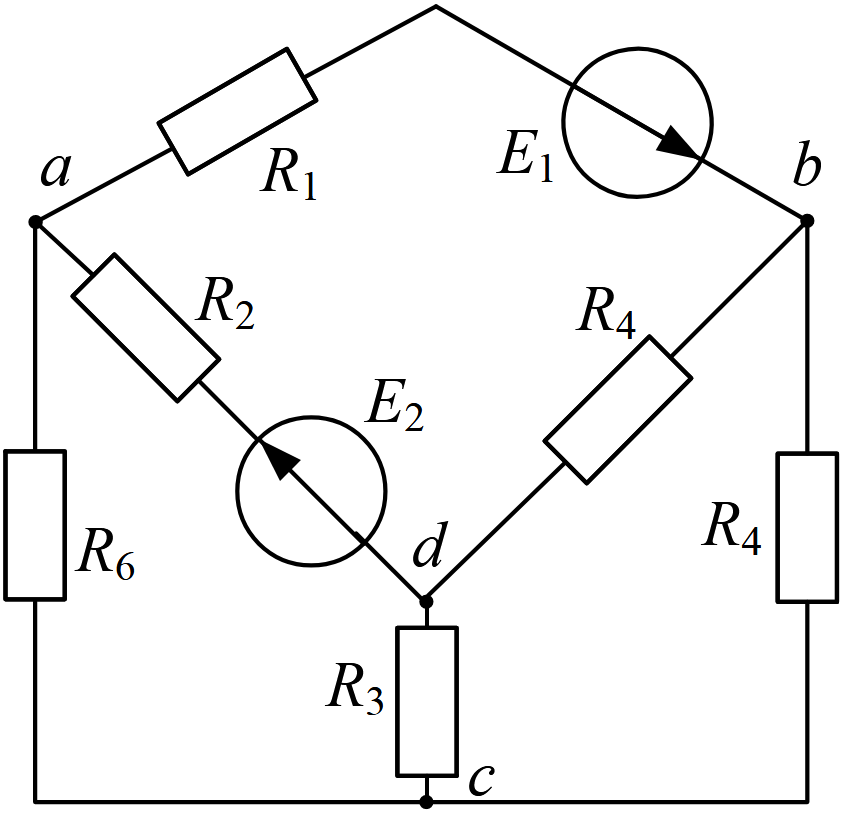
\includegraphics[width=0.7\textwidth]{images/30_task.png}
    \caption{схема для примера}
    \label{fig:example}
\end{figure}
Дано:
\begin{table}[H]
\centering
\begin{tabular}{|c|c|c|}
\hline
\textbf{Параметр} & \textbf{Обозначение} & \textbf{Значение} \\
\hline
Источник ЭДС 1 & $E_1$ & 30 В \\
\hline
Источник ЭДС 2 & $E_2$ & 10 В \\
\hline
Сопротивление 1 & $R_1$ & 3 Ом \\
\hline
Сопротивление 2 & $R_2$ & 4 Ом \\
\hline
Сопротивление 3 & $R_3$ & 10 Ом \\
\hline
Сопротивление 4 & $R_4$ & 4 Ом \\
\hline
Сопротивление 5 & $R_5$ & 6 Ом \\
\hline
Сопротивление 6 & $R_6$ & 3 Ом \\
\hline
\end{tabular}
\caption{Исходные данные для расчета}
\label{tab:initial_data}
\end{table}

\subsubsection{Задача 1. Контуры, узлы и ветви}
\textit{Необходимо посчитать для своей схемы количество узлов, ветвей и контуров, а также определить независимые контура и узлы.}

В данной схеме:
\begin{flushleft}
$q = 4$ (количество узлов) \\
$b = 6$ (количество ветвей) \\
$q-1 = 4-1 = 3$ (количество независимых узлов) \\
$n = 7$ (количество контуров) \\
$p = n-(q-1) = 7-(4-1) = 7-3 = 3$ (независимые контура)
\end{flushleft}

\begin{table}[H]
\centering
\begin{tabular}{|c|c|}
\hline
\textbf{Параметр} & \textbf{Значение} \\
\hline
Количество узлов (q) & 4 \\
\hline
Количество ветвей (b) & 6 \\
\hline
Количество независимых узлов (q-1) & 3 \\
\hline
Количество контуров (n) & 7 \\
\hline
Независимые контура (p) & 3 \\
\hline
\end{tabular}
\caption{Характеристики схемы}
\label{tab:circuit_characteristics}
\end{table}


\subsubsection{Задача 3. Анализ схемы на возможность упрощения. Метод эквивалентных преобразований}
\textit{Упростить схему методом эквивалентных преобразований и найти эквивалентное сопротивление.}

В данной схеме присутствует соедиинение как звездой, так и треугольником. Однако их преобразование только усложнит расчеты. Последовательно и параллельно соединенных резисторов в одной ветви нет. Поэтому упрощение схемы невозможно.


\subsubsection{Задача 4. Законы Кирхгофа}
\textit{Составить систему уравнений по законам Кирхгофа и решить её для определения токов в ветвях.}

\textbf{Решение:}

Расставим направление токов в ветвях и выберем необходимые нам независимые узлы. Это будут a,b,c.

Выберем 3 независимых контура для составления уравнений по 2-му закону Кирхгофа.

3-мя независимыми друг к другу контура являются adc, bdc, adb.

\begin{figure}[H]
    \centering
    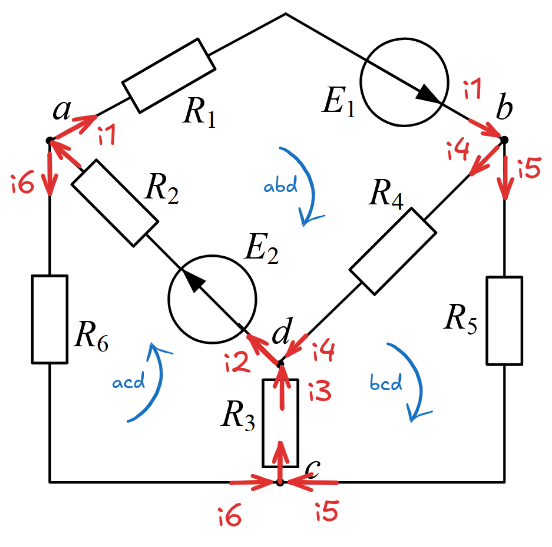
\includegraphics[width=0.7\textwidth]{images/Klaws_kontours_nodes.png}
    \caption{схема для примера}
    \label{fig:example}
\end{figure}

Можно заметить, что обозначение контуров через последовательность узлов однозначно определяет их направление и положение на схеме.


Составляем систему уравнений по законам Кирхгофа :
